\documentclass[12pt, a4paper]{article}

% ── Packages ────────────────────────────────────────────────────────────────
\usepackage[T1]{fontenc}
\usepackage[utf8]{inputenc}
\usepackage[english]{babel}
\usepackage{lmodern}
\usepackage{microtype}
\usepackage{geometry}
\geometry{margin=2.5cm}
\usepackage{graphicx}
\usepackage{float}
\usepackage{subcaption}
\usepackage{booktabs}
\usepackage{tabularx}
\usepackage{array}
\usepackage{hyperref}
\hypersetup{
  colorlinks=true,
  linkcolor=blue!60!black,
  citecolor=blue!60!black,
  urlcolor=blue!60!black
}
\usepackage{cite}
\usepackage{amsmath}
\usepackage{xcolor}
\usepackage{listings}
\usepackage{enumitem}
\usepackage{abstract}
\usepackage{titlesec}
\usepackage{fancyhdr}
\usepackage{setspace}
\usepackage{parskip}

% ── Formatting ───────────────────────────────────────────────────────────────
\setlength{\parindent}{0pt}
\setlength{\parskip}{6pt}
\onehalfspacing

\titleformat{\section}{\large\bfseries}{\thesection.}{0.5em}{}
\titleformat{\subsection}{\normalsize\bfseries}{\thesubsection.}{0.5em}{}

\pagestyle{fancy}
\fancyhf{}
\rhead{\small LEXIA --- Legal Design Journal}
\lhead{\small Vagnoni et al., 2026}
\cfoot{\thepage}

% ── Metadata ─────────────────────────────────────────────────────────────────
\title{
  \textbf{LEXIA: A Legal Design Approach to EU AI Act Compliance for Citizens}\\[0.5em]
  \large A Three-Layer Browser Extension Grounded in Human-Centred Design,\\
  Knowledge Graphs, and Explainable AI Extraction
}

\author{
  Simone Vagnoni\textsuperscript{1} \and
  [Co-author 2]\textsuperscript{1} \and
  [Co-author 3]\textsuperscript{1} \and
  [Co-author 4]\textsuperscript{1} \and
  [Co-author 5]\textsuperscript{1}
  \\[0.5em]
  \small\textsuperscript{1}[Institution], Bologna, Italy\\
  \small Submitted to the \textit{Legal Design Journal} ---
  \href{https://legaldesign-journal.com}{legaldesign-journal.com}
}

\date{May 2026}

% ─────────────────────────────────────────────────────────────────────────────
\begin{document}
\maketitle
\thispagestyle{fancy}

% ── Abstract ─────────────────────────────────────────────────────────────────
\begin{abstract}
\noindent
The EU AI Act (Regulation 2024/1689) grants citizens a set of enforceable rights --- the right to explanation, human oversight, AI transparency, and the right to lodge a complaint --- yet nearly two years after its entry into force, no major AI platform explicitly communicates these rights in its public-facing Terms of Service or Privacy Policy. This paper presents \textbf{LEXIA}, a browser extension that applies legal design principles to make AI Act compliance legible to citizens in real time. Drawing on the Legal Design Alliance's five core principles --- human-centred, proactive, effective, prototyping, and empirically evaluated --- LEXIA implements a three-layer architecture: a machine-readable Knowledge Graph built from Akoma Ntoso (AKN) XML legal sources, an Explainable AI extraction bridge powered by Azure OpenAI o4-mini, and a human-readable popup interface with adult and child-friendly reading modes. An empirical evaluation across five major platforms (OpenAI, Anthropic, X/Twitter, Klarna, Facebook) finds that all score red: none grants any of the six AI Act rights in its Privacy Policy. The findings are grounded in a transparent, per-concept scoring system traceable back to specific paragraph-level AKN eIds. We discuss how the design space for effective legal transparency --- contextual, multi-channel, layered --- informs both the tool's architecture and its citizen-facing interface, and outline future directions including LegalRuleML-based exception modelling and FrameNet-based clause tagging.

\vspace{0.5em}
\noindent\textbf{Keywords:} Legal design, EU AI Act, GDPR, explainable AI, browser extension, Knowledge Graph, citizens' rights, transparency, AKN, ontology
\end{abstract}

\vspace{1em}

% ─────────────────────────────────────────────────────────────────────────────
\section{Introduction}

The law creates rights. Tools make them real.

The EU AI Act (Regulation (EU) 2024/1689), in force since August 2024, is the world's first comprehensive legal framework for artificial intelligence. It grants citizens the right to explanation of AI-based decisions (Art.\ 86), human oversight of high-risk systems (Art.\ 14), disclosure of AI interaction (Art.\ 50), and the right to lodge a complaint with a market surveillance authority (Art.\ 85). These rights are grounded further in the General Data Protection Regulation (Regulation (EU) 2016/679), particularly Art.\ 22 on automated decision-making and Art.\ 17 on erasure.

The problem is not the absence of rights. It is the absence of communication. Legal texts are inaccessible to non-specialists. Corporate Terms of Service and Privacy Policies --- the documents that govern the daily interaction of millions of citizens with AI systems --- have not been updated to reflect the new legal framework. Citizens exercising rights they do not know they hold, against platforms that have not disclosed how those rights are fulfilled, cannot meaningfully participate in the legal system the AI Act intends to build.

This is precisely the gap that legal design is built to close. As articulated by the Legal Design Alliance, legal design \emph{"applies human-centered design to the world of law to enable desirable outcomes and prevent problems from arising"} \cite{lda2018}. It prioritises the point of view of the users of the law --- not of lawyers, courts, or regulators --- and demands that legal products be \emph{straightforward, engaging, and user-friendly}.

This paper presents \textbf{LEXIA}, a browser extension that embodies these principles in the context of AI regulation. LEXIA reads a platform's Privacy Policy, maps it against a formal ontology of EU AI Act and GDPR concepts using an LLM-based extraction pipeline, and displays the findings as a traffic-light semaphore with per-right and per-risk cards, each traceable to the exact AKN paragraph in EUR-Lex. A child-friendly mode provides an alternative interface for younger users. When a user visits a supported site for the first time each day, LEXIA proactively notifies them of the compliance status --- without requiring any action on the user's part.

The paper is structured as follows. Section~2 reviews the legal design literature and situates LEXIA within it. Section~3 describes the system architecture. Section~4 presents the methodology. Section~5 reports results from an evaluation of five major AI platforms. Section~6 discusses the findings in legal design terms. Section~7 outlines future directions. Section~8 concludes.

% ─────────────────────────────────────────────────────────────────────────────
\section{Legal Design Background and Related Work}

\subsection{Legal Design Principles}

The Legal Design Alliance's Manifesto \cite{lda2018} defines five core principles that guide the design of legal products and services. We use these as an evaluative framework for LEXIA.

\textbf{Human-centred.} Legal design starts from the needs and abilities of the users of the law, not from the needs of lawyers and courts. LEXIA is designed for citizens --- not compliance officers. Its interface presents findings in plain language, avoids legal jargon, and offers a dedicated child-friendly mode with emoji, star ratings, and simplified explanations.

\textbf{Proactive.} Legal design drives desirable outcomes rather than merely dealing with the consequences of failure. LEXIA notifies users on their first visit to a supported site each day, without requiring them to actively seek information. The badge on the extension icon shows the compliance score at a glance, before the user has even opened the popup.

\textbf{Effective.} Legal products should enable people to understand and do the right thing easily, without requiring considerable investments of time, money, effort, or expertise. LEXIA reduces the cognitive cost of compliance checking to a single click, and provides AKN-linked legal sources for users who wish to verify findings.

\textbf{Prototyping.} Solutions should be developed through quick rounds of iteration and experimentation. LEXIA was built as a hackathon prototype, tested against five live platforms, and iterated on the basis of empirical extraction results.

\textbf{Empirically evaluated.} LEXIA produces quantitative outputs --- a 0--100 compliance score with a per-concept breakdown --- that make the current state of platform compliance measurable, comparable, and auditable.

\subsection{Transparency as Legal Design Object}

The GDPR already established transparency as a design constraint. Art.\ 12(7) requires that information relating to processing be provided \emph{"in a concise, transparent, intelligible and easily accessible form, using clear and plain language."} This obligation transformed the privacy notice from a legal artefact into a design artefact --- and produced a wave of research and practice on how to design effective transparency \cite{schaub2015, edpb2019}.

Schaub et al.\ \cite{schaub2015} define a design space for effective privacy notices across four dimensions: timing (when the notice is shown), channel (where it appears), modality (how it is presented), and choice (what control it affords). They argue that effective transparency must be \emph{contextual} (delivered at the moment of relevance), \emph{multi-channel} (differentiated across media), and \emph{layered} (balancing completeness and understandability). LEXIA is explicitly designed around these three axes: it is contextual (triggered at the moment of site visit), multi-channel (browser extension badge, slide-in notification, popup), and layered (traffic-light semaphore → per-concept cards → AKN full text).

The trajectory from privacy notices to AI system documentation is not a discontinuity but an extension. The AI Act imposes on AI deployers the same design obligation that the GDPR imposed on data controllers: to make legal information accessible to the people it concerns. LEXIA operationalises this obligation at the citizen-facing layer.

\subsection{Related Work}

\textbf{ToSDR} (Terms of Service; Didn't Read) \cite{tosdr} is the closest existing tool: it crowdsources human evaluations of Terms of Service and presents findings in plain language with letter grades. LEXIA differs in three ways: it grounds every finding in a specific AKN legal source, it is automated (rather than crowdsourced), and it targets the EU AI Act specifically rather than general consumer rights.

\textbf{Polisis} \cite{harkous2018} uses neural networks to analyse Privacy Policies and visualise their structure. It does not produce legal citations and does not target the AI Act.

\textbf{CLAUDETTE} \cite{lippi2019} applies NLP to detect potentially unfair clauses in Terms of Service, using GDPR as the normative reference. LEXIA extends this approach to the AI Act and adds a citizen-facing visualisation layer.

None of these tools implements the three-layer architecture that connects machine-readable legal ontologies, LLM-based extraction, and a citizen-facing interface within a single, deployable browser extension.

% ─────────────────────────────────────────────────────────────────────────────
\section{System Architecture}

LEXIA is inspired by the Creative Commons model: three representation layers, each readable by a different audience.

\begin{figure}[H]
  \centering
  \includegraphics[width=\textwidth]{../LEXIA_diagram.png}
  \caption{LEXIA system architecture. Three layers: machine-readable Knowledge Graph (Layer 1), XAI extraction bridge (Layer 2), and human-readable browser extension (Layer 3).}
  \label{fig:architecture}
\end{figure}

\subsection{Layer 1 — Machine-Readable Knowledge Graph}

The Knowledge Graph is built from two Akoma Ntoso (AKN) XML files: the EU AI Act (CELEX 32024R1689) and the GDPR (CELEX 32016R0679). Python's ElementTree parser extracts paragraph text at each paragraph-level eId (e.g.\ \texttt{chp\_IX\_\_sec\_4\_\_art\_86\_\_para\_1}), preserving the authoritative wording.

The graph integrates four ontologies:
\begin{itemize}[noitemsep]
  \item \textbf{AIRO} (AI Risk Ontology) \cite{airo}: risk levels and AI system types
  \item \textbf{DPV EU-AIAct} \cite{dpv}: system types, roles, and compliance concepts
  \item \textbf{VAIR} \cite{vair}: risk vocabulary
  \item \textbf{PrOnto} \cite{pronto}: rights and obligations iconography
\end{itemize}

The concept--AKN mapping (\texttt{concept\_akn\_mapping.json}) defines \textbf{10 concept IDs} --- 6 rights and 4 risks --- each linked to its primary and secondary AKN legal sources with character-level highlight offsets and EUR-Lex URLs.

\subsection{Layer 2 — XAI Extraction Bridge}

For each platform, the pipeline:

\begin{enumerate}[noitemsep]
  \item Retrieves the Privacy Policy from the pre-downloaded ToSDR corpus or via live scraping with English-language headers (\texttt{tos\_scraper.py})
  \item Queries the Wikidata SPARQL endpoint to determine the platform's AIRO system type, which calibrates risk weights (\texttt{wikidata\_client.py})
  \item Passes the policy text (up to 14,000 characters) to Azure OpenAI o4-mini with a structured prompt that lists all 10 concept IDs and their legal labels (\texttt{tos\_extractor.py})
  \item Computes a 0--100 compliance score using a weighted penalty/bonus formula calibrated by system type (\texttt{semaphore.py})
\end{enumerate}

The scoring formula applies risk penalties when a risk practice is confirmed in the ToS, right-violation penalties (at $1.5\times$ base weight) when a right is explicitly blocked, and an uncertainty cost (40\% of the weight) when a concept is absent from the document. Granted rights contribute a bonus at 30\% of their weight. The formula is:

\[
\text{score} = \text{clamp}\!\left(100 - \sum_i p_i + 0.3 \sum_j b_j,\ 0,\ 100\right)
\]

where $p_i$ are penalties and $b_j$ are right bonuses. The score maps to three semaphore states: green ($\geq 70$), orange ($\geq 40$), red ($< 40$).

\subsection{Layer 3 — Human-Readable Interface}

The Chrome Manifest V3 browser extension consists of:

\begin{itemize}[noitemsep]
  \item A \textbf{service worker} (\texttt{background.js}) that fetches compliance data on tab activation, sets a coloured score badge on the extension icon, and sends data to the content script
  \item A \textbf{content script} (\texttt{content.js}) that injects a slide-in notification banner on the first visit to a supported site each day
  \item A \textbf{popup} (\texttt{popup.html / popup.js}) with semaphore, per-concept cards, and an AKN slide-in panel showing highlighted article text with EUR-Lex links
\end{itemize}

The popup implements two reading modes: \textbf{adult mode} (legally precise, with article citations) and \textbf{child-friendly mode} (plain language, emoji, star ratings, large icons without borders). Screenshots of both modes are shown in Figure~\ref{fig:screenshots}.

\begin{figure}[H]
  \centering
  \begin{subfigure}[t]{0.48\textwidth}
    \centering
    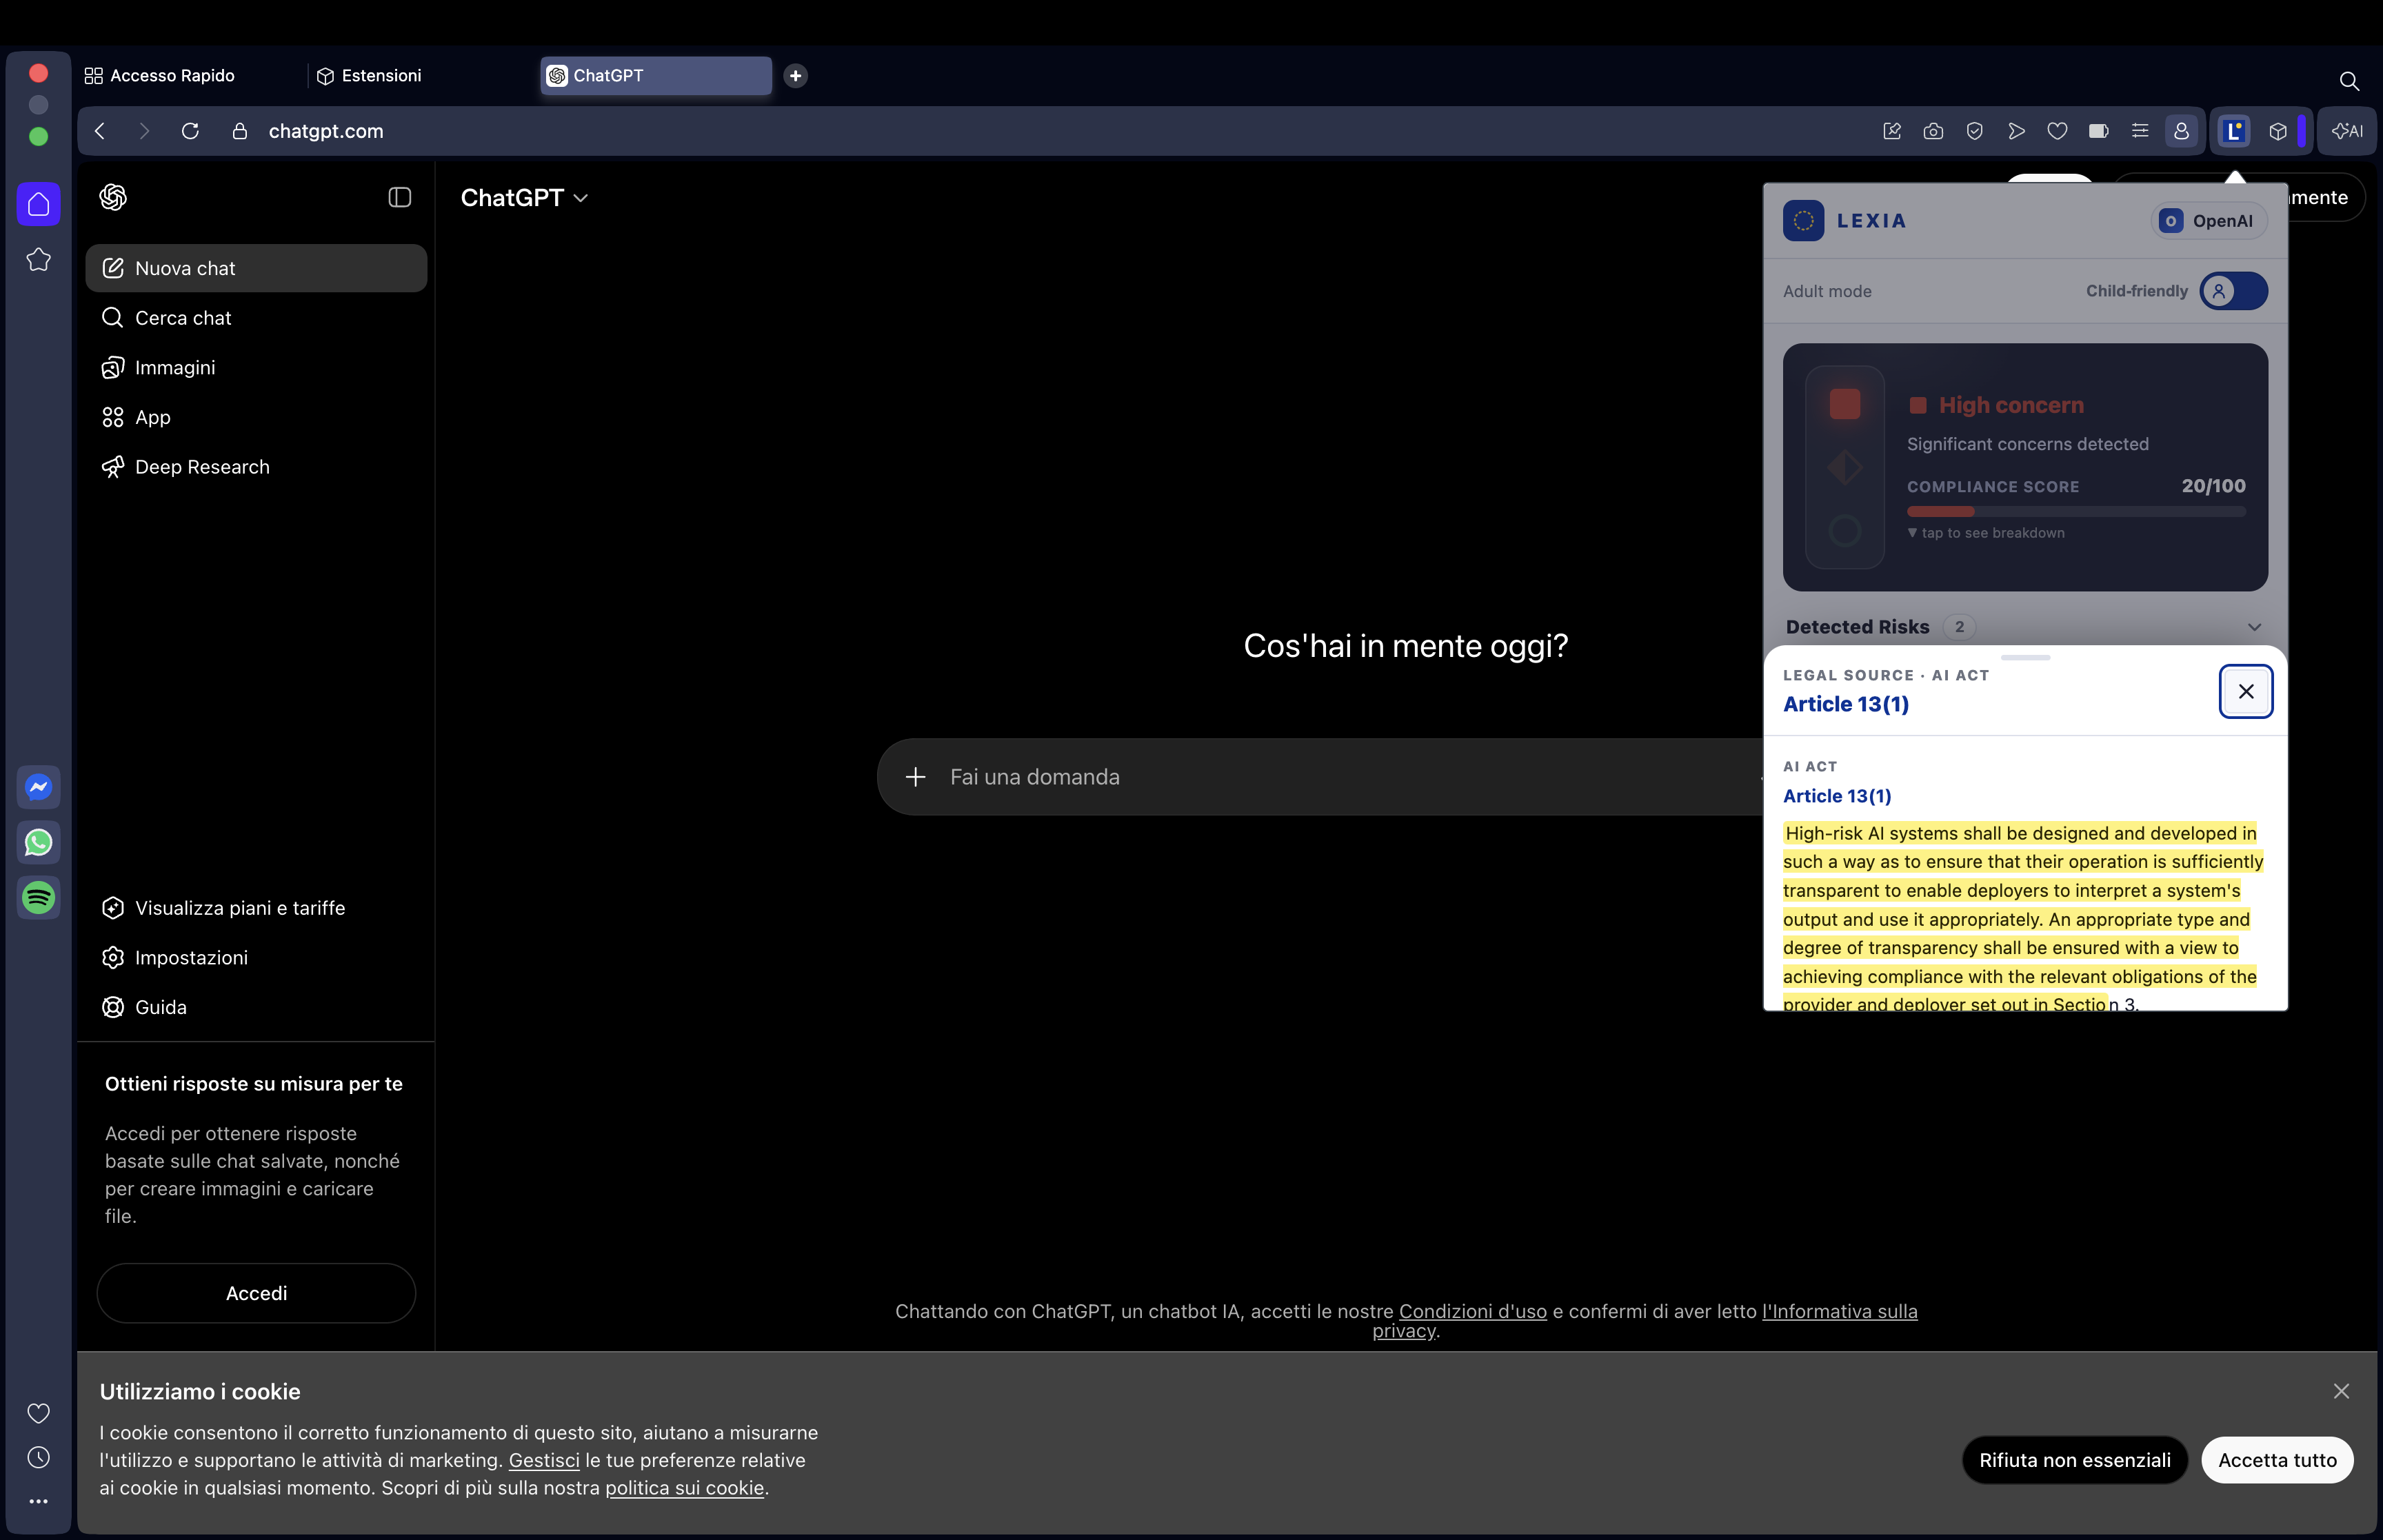
\includegraphics[width=\textwidth]{../screenshot_adult_mode.png}
    \caption{Adult mode: traffic-light semaphore, per-concept cards with AKN citations, score breakdown.}
  \end{subfigure}
  \hfill
  \begin{subfigure}[t]{0.48\textwidth}
    \centering
    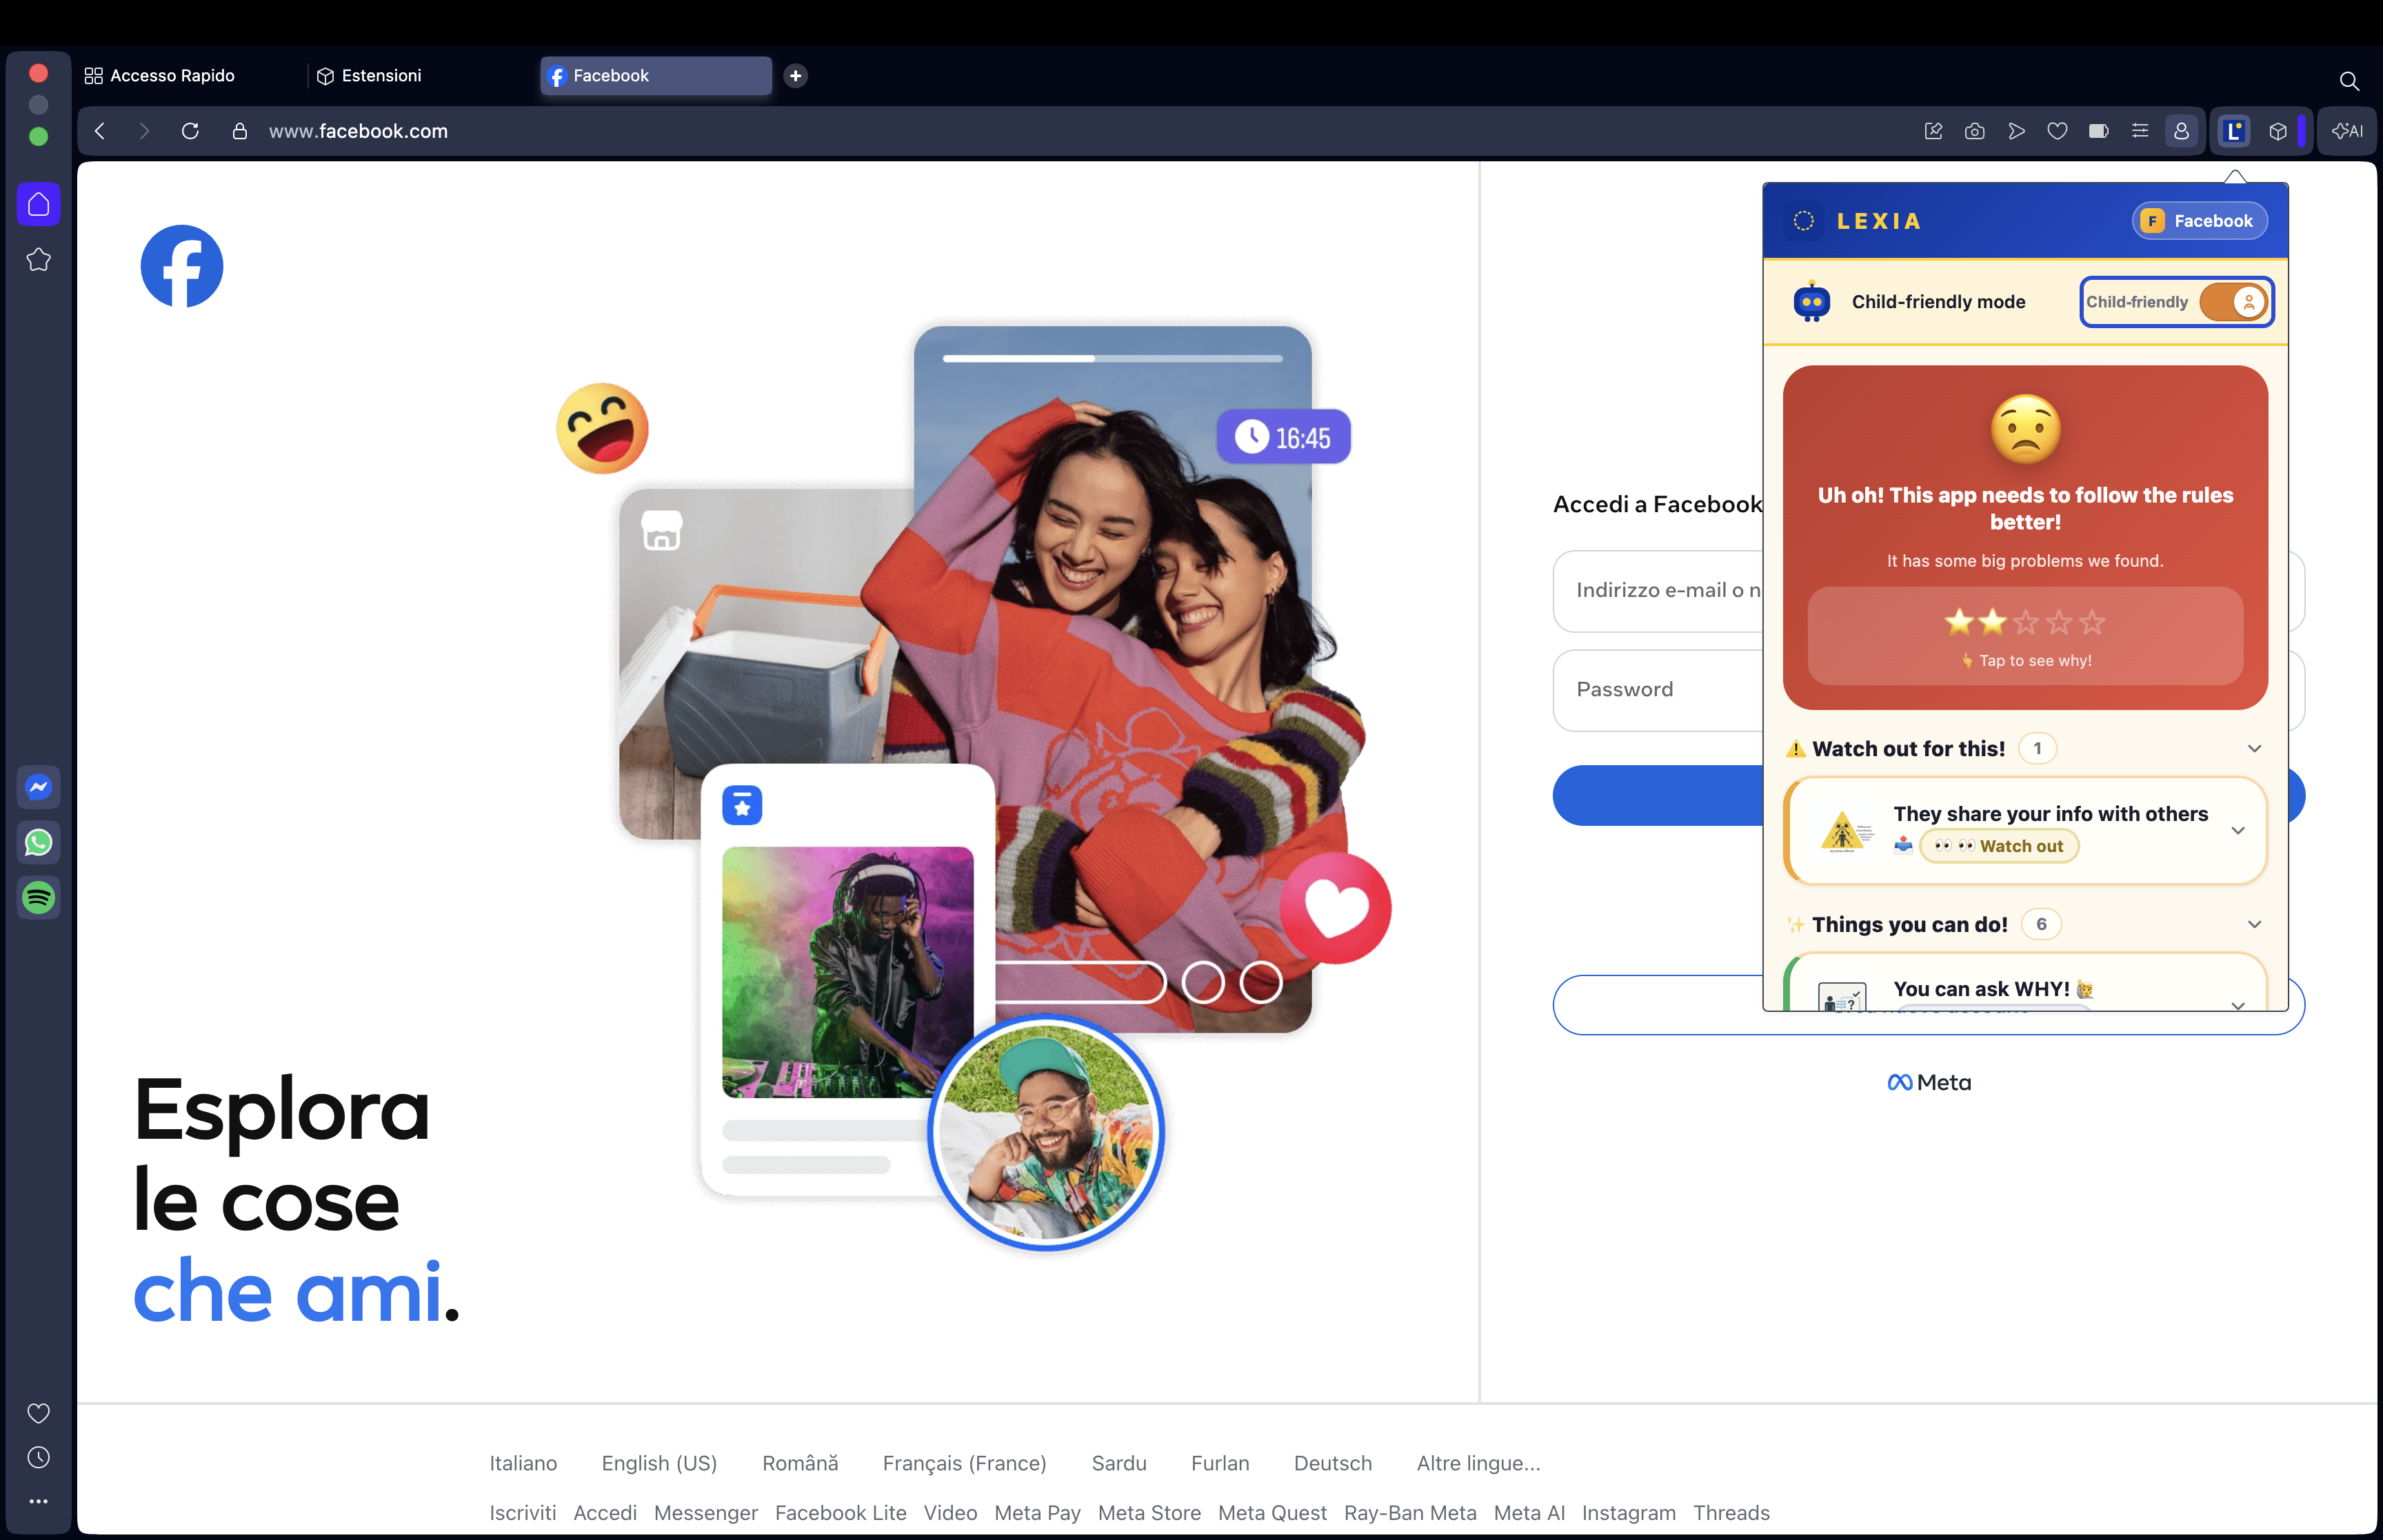
\includegraphics[width=\textwidth]{../screenshot_child_mode.png}
    \caption{Child-friendly mode: emoji semaphore with star rating, simplified labels, large icons.}
  \end{subfigure}
  \caption{LEXIA popup interface in adult and child-friendly reading modes.}
  \label{fig:screenshots}
\end{figure}

% ─────────────────────────────────────────────────────────────────────────────
\section{Methodology}

\subsection{Dataset}

We use four data sources:

\textbf{AKN XML files.} The authoritative legislative text of the EU AI Act (32024R1689) and GDPR (32016R0679) from the EUR-Lex Publications Office, structured with paragraph-level eId anchors.

\textbf{ToSDR corpus.} Pre-downloaded Privacy Policies and Terms of Service from the ToSDR dataset \cite{tosdr}, covering OpenAI, Anthropic, Facebook, Klarna, and X/Twitter. Each document is stored as structured JSON with \texttt{text}, \texttt{url}, and \texttt{updated\_at} fields. The combined text per platform is capped at 14,000 characters.

\textbf{Wikidata.} SPARQL queries retrieve each platform's \texttt{P31} (instance of) value, mapped to an AIRO system type to calibrate risk scoring.

\textbf{Concept--AKN mapping.} A hand-crafted mapping of 10 concept IDs to their AKN legal sources, serving as the shared interface between the Knowledge Graph, the extraction pipeline, and the frontend.

\subsection{Extraction Prompt Design}

The extraction prompt is constructed deterministically from \texttt{concept\_akn\_mapping.json}. The model receives:
\begin{itemize}[noitemsep]
  \item The full list of 10 concept IDs with their legal labels and categories (right vs.\ risk)
  \item A three-value status schema: \texttt{granted} / \texttt{violated} / \texttt{unknown}
  \item Explicit definitional rules distinguishing confirmed practice from prohibited practice from absence
  \item A special rule for \texttt{no\_ai\_disclosure}: if the ToS does not mention AI interaction disclosure, status is \texttt{granted} (risk present)
\end{itemize}

The model returns a JSON object with \texttt{status}, \texttt{evidence} (verbatim quote, $\leq 120$ characters), and \texttt{confidence} for each concept. A repair prompt is attempted on parse failure before falling back to all-unknown.

\subsection{Limitations}

The 14,000-character truncation introduces a systematic downward bias in rights detection: data subject rights disclosures typically appear in the final sections of long privacy policies. Facebook's full Privacy Policy, for instance, exceeds 200,000 characters; the analysed excerpt represents less than 7\% of the full document. The \texttt{unknown} count is therefore likely inflated, and the true compliance picture may be marginally better than scores suggest. A more robust evaluation would require section-targeted retrieval and human verification.

% ─────────────────────────────────────────────────────────────────────────────
\section{Results}

Table~\ref{tab:results} summarises the compliance scores for the five platforms evaluated.

\begin{table}[H]
\centering
\caption{LEXIA compliance scores for five major AI platforms (May 2026). All platforms score red. No platform explicitly grants any of the six EU AI Act rights in its public legal documentation.}
\label{tab:results}
\begin{tabularx}{\textwidth}{lXccc}
\toprule
\textbf{Platform} & \textbf{System Type} & \textbf{Score} & \textbf{Semaphore} & \textbf{Rights Granted} \\
\midrule
OpenAI / ChatGPT  & conversational\_ai & 20/100 & \textcolor{red}{Red}    & 0/6 \\
X / Twitter       & social\_network    & 11/100 & \textcolor{red}{Red}    & 0/6 \\
Klarna            & marketplace        & 22/100 & \textcolor{red}{Red}    & 0/6 \\
Anthropic / Claude & conversational\_ai & 0/100  & \textcolor{red}{Red}    & 0/6 \\
Facebook          & social\_network    & 35/100 & \textcolor{red}{Red}    & 0/6 \\
\bottomrule
\end{tabularx}
\end{table}

\textbf{The primary finding is unambiguous}: no platform grants any of the six EU AI Act rights in its publicly available legal documents. All six --- \texttt{right\_explanation} (Art.\ 86), \texttt{right\_human\_oversight} (Art.\ 14), \texttt{right\_ai\_transparency} (Art.\ 50), \texttt{right\_complaint} (Art.\ 85), \texttt{right\_erasure} (GDPR Art.\ 17), and \texttt{right\_contest} (GDPR Art.\ 22) --- are marked \texttt{unknown} across all five platforms.

Risk detection produces documentary evidence. OpenAI's Privacy Policy explicitly states: \emph{"we may use Content you provide us to improve our services, including to train the models that power ChatGPT"} --- triggering \texttt{training\_on\_user\_data}. Facebook confirms profiling of user behaviour from third-party activity signals. Anthropic discloses data sharing with sub-processors and analytics providers, triggering three risk categories.

The \texttt{no\_ai\_disclosure} risk was not confirmed for any platform --- all five mention AI interaction to some degree, satisfying the basic transparency obligation of Art.\ 50(1).

\textbf{The Anthropic paradox}: Anthropic scores lowest (0/100) despite having the most detailed Privacy Policy. A more transparent document exposes more detectable risk signals. This reveals a tension in compliance-by-transparency approaches: disclosed-and-unmitigated risk is penalised more than undisclosed risk. Future scoring should distinguish between disclosed-and-mitigated and disclosed-and-unmitigated practices.

% ─────────────────────────────────────────────────────────────────────────────
\section{Discussion}

\subsection{LEXIA as Legal Design}

LEXIA instantiates each of the five legal design principles in a concrete technical choice.

\emph{Human-centred}: The child-friendly mode was designed from scratch with non-specialist users in mind, replacing legal terminology with plain language, emoji status badges, and star ratings. The semaphore in child mode shows a large emoji face (😟 / 🤔 / 😊) rather than a geometric traffic light, and the score breakdown is explained as a point system rather than a formula.

\emph{Proactive}: The slide-in notification banner appears automatically on the first visit to a supported site each day. The score badge on the extension icon is updated on every tab change. Citizens receive compliance information without seeking it.

\emph{Effective}: The popup collapses findings into a single semaphore that communicates both by colour and by shape (satisfying WCAG 2.1 AA colour-independence requirements), supported by expanding cards for users who want detail, and an AKN panel for users who want the authoritative legal text.

\emph{Prototyping}: The system was built and tested iteratively during a hackathon. Each pipeline run against a live platform produced output that informed prompt revisions, scoring calibration, and interface adjustments.

\emph{Empirically evaluated}: The 0--100 score, with a per-concept breakdown and a human-readable formula (\texttt{100 − 80 pts penalties + 0 pts bonus = 20/100}), makes compliance measurable, comparable across platforms, and auditable by the user.

\subsection{The Layered Design of Legal Transparency}

Schaub et al.'s design space \cite{schaub2015} describes effective privacy notices as contextual, multi-channel, and layered. LEXIA maps directly onto these dimensions:

\textbf{Contextual}: Information is delivered at the moment of site visit, not in an abstract legal repository.

\textbf{Multi-channel}: Three distinct channels carry the same information at different depths --- the badge (one number), the notification banner (one sentence + emoji), the popup (full per-concept breakdown with evidence quotes), and the AKN panel (full legal text with highlighted passage).

\textbf{Layered}: The interface moves from the most compressed representation (traffic light) to the most complete (AKN full text). Users can stop at any layer. The child mode provides a parallel compressed layer for a different audience.

This architecture reflects what Hagan describes as the shift from \emph{redesigning legal information} to \emph{redesigning entire systems} \cite{hagan2017}: LEXIA is not a better privacy notice. It is a system that reads privacy notices on behalf of citizens and translates them into actionable signals.

\subsection{The Transparency Gap as a Regulatory Finding}

The unanimous red score across five major platforms is not a finding about their internal compliance practices. It is a finding about \emph{communication}: the EU AI Act creates rights, but the platforms that must honour them have not told their users that those rights exist. This failure at the communication layer is precisely what Art.\ 13 AI Act requires to be corrected for high-risk systems.

The Italian Data Protection Authority's white paper on legal design \cite{garante2025} demonstrates that regulatory bodies are increasingly aware that the form of legal communication matters as much as its content. LEXIA applies the same insight to the AI Act: compliance is not achieved until citizens can verify it.

% ─────────────────────────────────────────────────────────────────────────────
\section{Future Directions}

Three directions define the roadmap.

\textbf{LegalRuleML-based exception modelling.} The current pipeline treats rights as binary signals. A legally adequate model must handle exceptions and derogations: Art.\ 50(1) exempts law enforcement AI from the disclosure obligation; Art.\ 86(2) limits the right to explanation where national law provides otherwise. Encoding these conditional structures requires \textbf{LegalRuleML} \cite{legalruleml}, the OASIS standard for machine-readable legal rules, which allows exceptions and defeasibility to be represented formally and reasoned over. This would allow LEXIA to determine not only whether a right exists in principle, but whether a specific exception applies to a given platform's context.

\textbf{FrameNet-based clause tagging.} The current pipeline treats ToS text as unstructured. Structured extraction using \textbf{frame semantics (FrameNet)} \cite{fillmore2002} would identify the full argument structure of legal clauses --- who does what to whom, under what conditions. Tagging ToS sentences with frames such as \emph{Data\_Transfer}, \emph{Consent\_Withdrawal}, or \emph{Automated\_Decision} would improve precision, reduce false negatives from paraphrased rights grants, and produce clause-level outputs. Combined with LegalRuleML, this would close the gap between raw text and traceable legal reasoning.

\textbf{Extended platform coverage and technical file access.} Extending coverage to the full 27-concept ontology requires access to technical files, conformity assessments, and model cards that become available as Art.\ 53 and Art.\ 55 obligations are enforced. This would allow LEXIA to address the most serious risk categories currently beyond citizen-facing access.

% ─────────────────────────────────────────────────────────────────────────────
\section{Conclusion}

LEXIA demonstrates that formal legal ontologies, structured LLM extraction, and human-centred design can be combined into a working tool that makes EU AI Act compliance legible to citizens at the moment of interaction with AI systems. The core empirical finding is also a legal design finding: in May 2026, nearly two years after the EU AI Act entered into force, no major AI platform explicitly grants citizens the rights the law creates. The gap is not technical. It is a gap in legal communication --- and closing it requires both better tools and stronger enforcement of the disclosure obligations the law already contains.

LEXIA is released under a CC-BY 4.0 licence. Source code, data, and the full extension are available at: \url{https://github.com/glongo01/LEGALDESIGNHACKATHON2026}

% ─────────────────────────────────────────────────────────────────────────────
\begin{thebibliography}{99}

\bibitem{lda2018}
Legal Design Alliance.
\newblock \emph{Legal Design Manifesto}.
\newblock Legal Design Alliance, 2018.
\newblock \url{https://www.legaldesignalliance.org/}

\bibitem{schaub2015}
F.\ Schaub, R.\ Balebako, A.\ Durity, and L.\ Cranor.
\newblock A design space for effective privacy notices.
\newblock In \emph{Proceedings of the Eleventh Symposium on Usable Privacy and
Security (SOUPS 2015)}, pages 1--17, 2015.

\bibitem{edpb2019}
European Data Protection Board.
\newblock \emph{Guidelines 4/2019 on Article 25: Data Protection by Design and
by Default}.
\newblock EDPB, 2019.
\newblock \url{https://edpb.europa.eu/}

\bibitem{hagan2017}
M.\ Hagan.
\newblock \emph{Law by Design}.
\newblock Legal Design Lab, Stanford University, 2017.
\newblock \url{https://lawbydesign.co/}

\bibitem{garante2025}
Creative Commons Italy and Garante per la Protezione dei Dati Personali.
\newblock \emph{White Paper --- Rendere le informative privacy più
comprensibili: Il legal design come approccio rivolto all'utente}.
\newblock Garante Privacy, 2025.
\newblock \url{https://www.garanteprivacy.it/temi/creative-commons}

\bibitem{tosdr}
ToS;DR Project.
\newblock \emph{Terms of Service; Didn't Read}.
\newblock \url{https://tosdr.org/}

\bibitem{harkous2018}
H.\ Harkous, K.\ Fawaz, R.\ Lebret, F.\ Schaub, K.\ Shin, and K.\ Aberer.
\newblock Polisis: Automated analysis and presentation of privacy policies
using deep learning.
\newblock In \emph{Proceedings of the 27th USENIX Security Symposium}, 2018.

\bibitem{lippi2019}
M.\ Lippi, P.\ Palka, G.\ Contissa, F.\ Lagioia, H.-W.\ Micklitz,
G.\ Sartor, and P.\ Torroni.
\newblock {CLAUDETTE}: An automated detector of potentially unfair clauses in
online terms of service.
\newblock \emph{Artificial Intelligence and Law}, 27(2):117--139, 2019.

\bibitem{airo}
D.\ Golpayegani, H.\ Pandit, and D.\ Lewis.
\newblock {AIRO}: An ontology for representing {AI} risks.
\newblock \emph{Semantic Web Journal}, 2023.
\newblock \url{https://w3id.org/airo}

\bibitem{dpv}
H.\ Pandit et al.
\newblock {DPV} {EU-AIAct} Extension.
\newblock Data Privacy Vocabulary Community Group, W3C, 2024.
\newblock \url{https://w3id.org/dpv/legal/eu/aiact}

\bibitem{vair}
D.\ Golpayegani, H.\ Pandit, and D.\ Lewis.
\newblock {VAIR}: Vocabulary for {AI} Risks.
\newblock 2023.
\newblock \url{https://w3id.org/vair}

\bibitem{pronto}
M.\ Palmirani, G.\ Governatori, A.\ Rotolo, S.\ Tabet, H.\ Boley, and
A.\ Paschke.
\newblock {PrOnto}: Privacy ontology for legal reasoning.
\newblock In \emph{e-Democracy 2018}, pages 139--152. Springer, 2018.

\bibitem{legalruleml}
M.\ Palmirani, G.\ Governatori, A.\ Rotolo, S.\ Tabet, H.\ Boley, and
A.\ Paschke.
\newblock {LegalRuleML}: {XML}-based rules and norms.
\newblock \emph{Rule-Based Reasoning, Programming, and Applications}, 2011.
\newblock OASIS Standard: \url{https://docs.oasis-open.org/legalruleml/}

\bibitem{fillmore2002}
C.\ Fillmore and C.\ Baker.
\newblock Frame semantics for {NLP}.
\newblock In \emph{Proceedings of the NAACL-2001 Workshop on Linguistic
Knowledge Acquisition and Representation}, 2002.
\newblock {FrameNet}: \url{https://framenet.icsi.berkeley.edu/}

\bibitem{rossi2026}
A.\ Rossi.
\newblock Legal design --- a primer.
\newblock Lecture, Hackathon LLM Legal Design XAI \& Rights, Bologna, 30 May
2026. Scuola Superiore S.\ Anna.

\end{thebibliography}

\end{document}
